\begin{itemize}
    \item “bottom-up” strategy
    \item iteratively solve smaller problems to solve progressively bigger problems
    \item Overlapping subproblems
    \item answers to smaller problems are stored in a table
    \item Example: Fibonacci
\end{itemize}

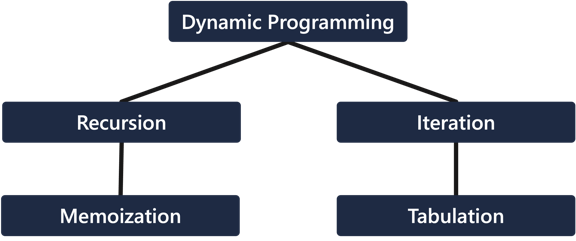
\includegraphics[width = \linewidth]{src/7_dp/images/dp.png}

Convert code from recursive to dynamic programming:
\begin{itemize}
    \item Look for repeating subproblems
    \item look for an optimal substructure to the solution – how does the answer of the problem depend on the answer of the subproblems?
    \item Should the answers of the subproblems be stored in a list? A table?
    \item Flip the recursive implementation around to implement a bottom-up, iterative solution.
\end{itemize}

{\centering \underline{\textbf{Example: dynamic programming approach to Fibonacci}} \par}
\lstinputlisting{src/7_dp/code/fibonacci.py}
